\section{Justifications of using \texttt{deepspeed-stage-2}}
\label{sub:justifications_of_deepspeed_2}
Eight A100 GPUs support the following configurations:
\begin{itemize}
    \item Full fine-tuning with an 8k context window using Fully Sharded Data Parallel (FSDP). 
    \item 6k context window with full attention using \texttt{deepspeed-stage-2}.
    \item 32k context window with full attention using \texttt{accelerate} and \texttt{deepspeed-stage-3-offload}. However, saving models in this configuration encountered version incompatibility issues and we haven't found solutions online. 
\end{itemize}
Based on these trails, we do not scale up the model with \texttt{deepspeed-stage-3-offload} or FSDP, but choose to use \texttt{deepspeed-stage-2} and set the cross-attention to be of the shape 2048 by 14848. 

\section{Experiments on datasets NaturalQA}

\subsection{Knowledge Retention Experiments on NaturalQA}
\label{sub:knowledge_retention_nqa}
The results of knowledge retention experiments on NaturalQA are shown in Figure \ref{fig:knowledge-retention-nqa}. 

\begin{figure}[h!]
    \centering
    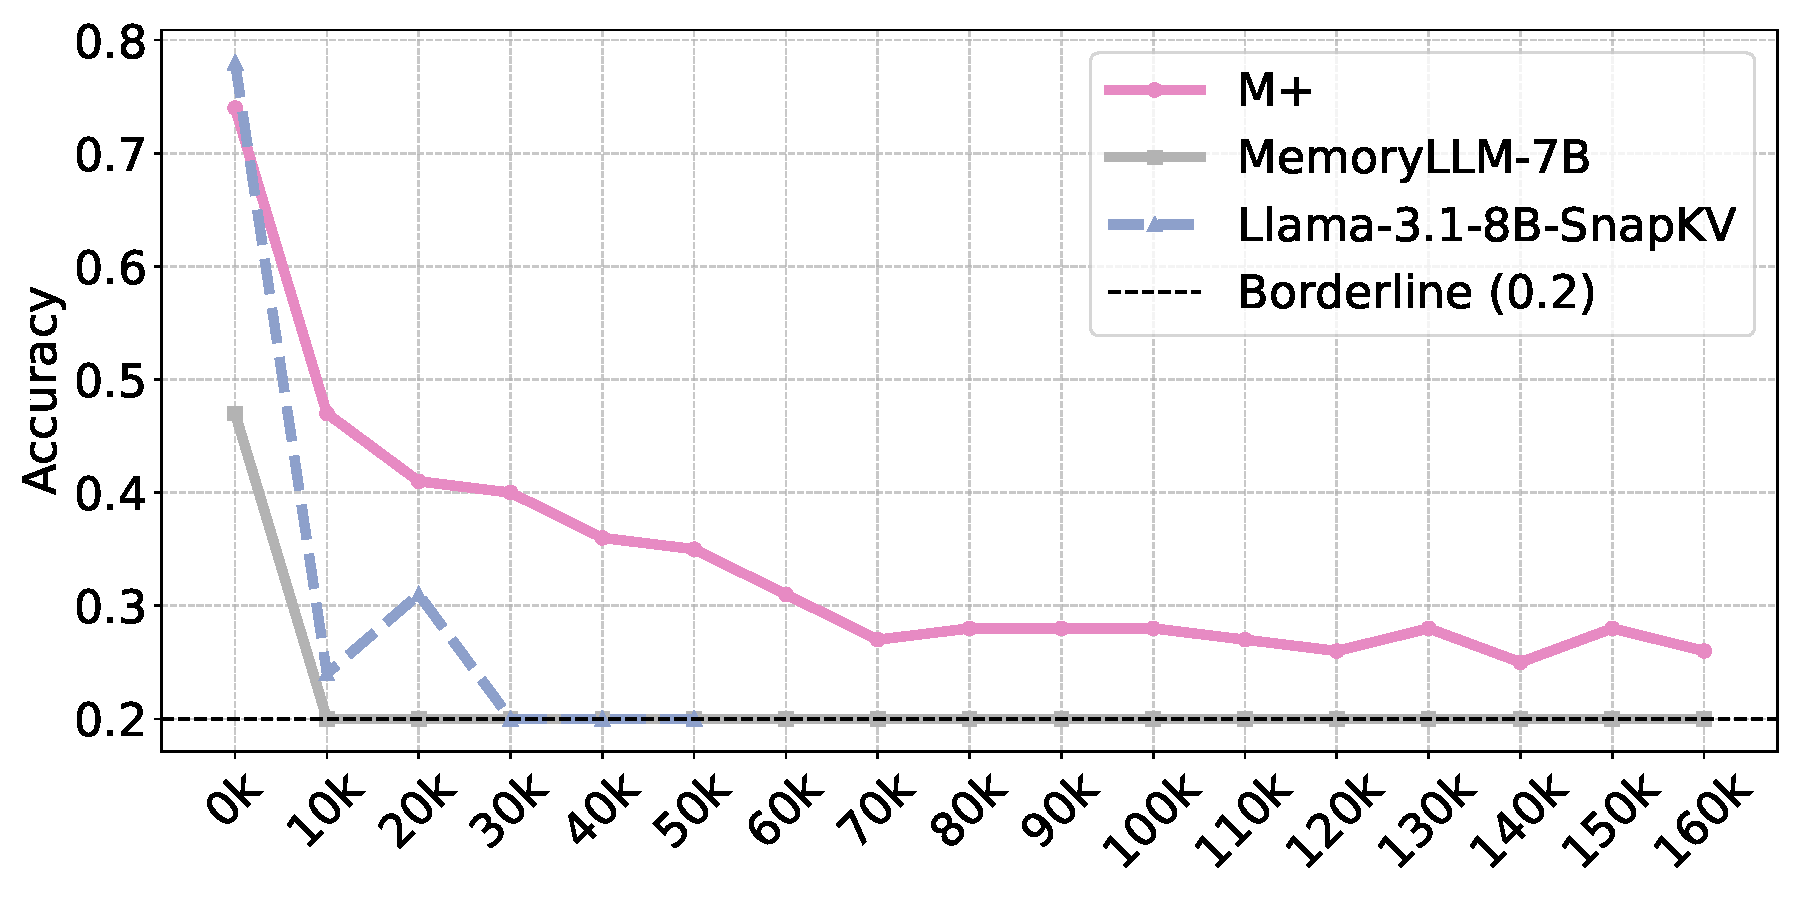
\includegraphics[width=0.6\linewidth]{figures/nqa.pdf}
    \caption{Knowledge Retention Results on NaturalQA.}
    \label{fig:knowledge-retention-nqa}
\end{figure}

\subsection{Ablation Study on NaturalQA}
\label{sub:ablation_study_naturalqa}
The results of ablation study on NaturalQA are shown in Figure \ref{fig:nqa_ablation}.

\begin{figure}[h!]
\centering
    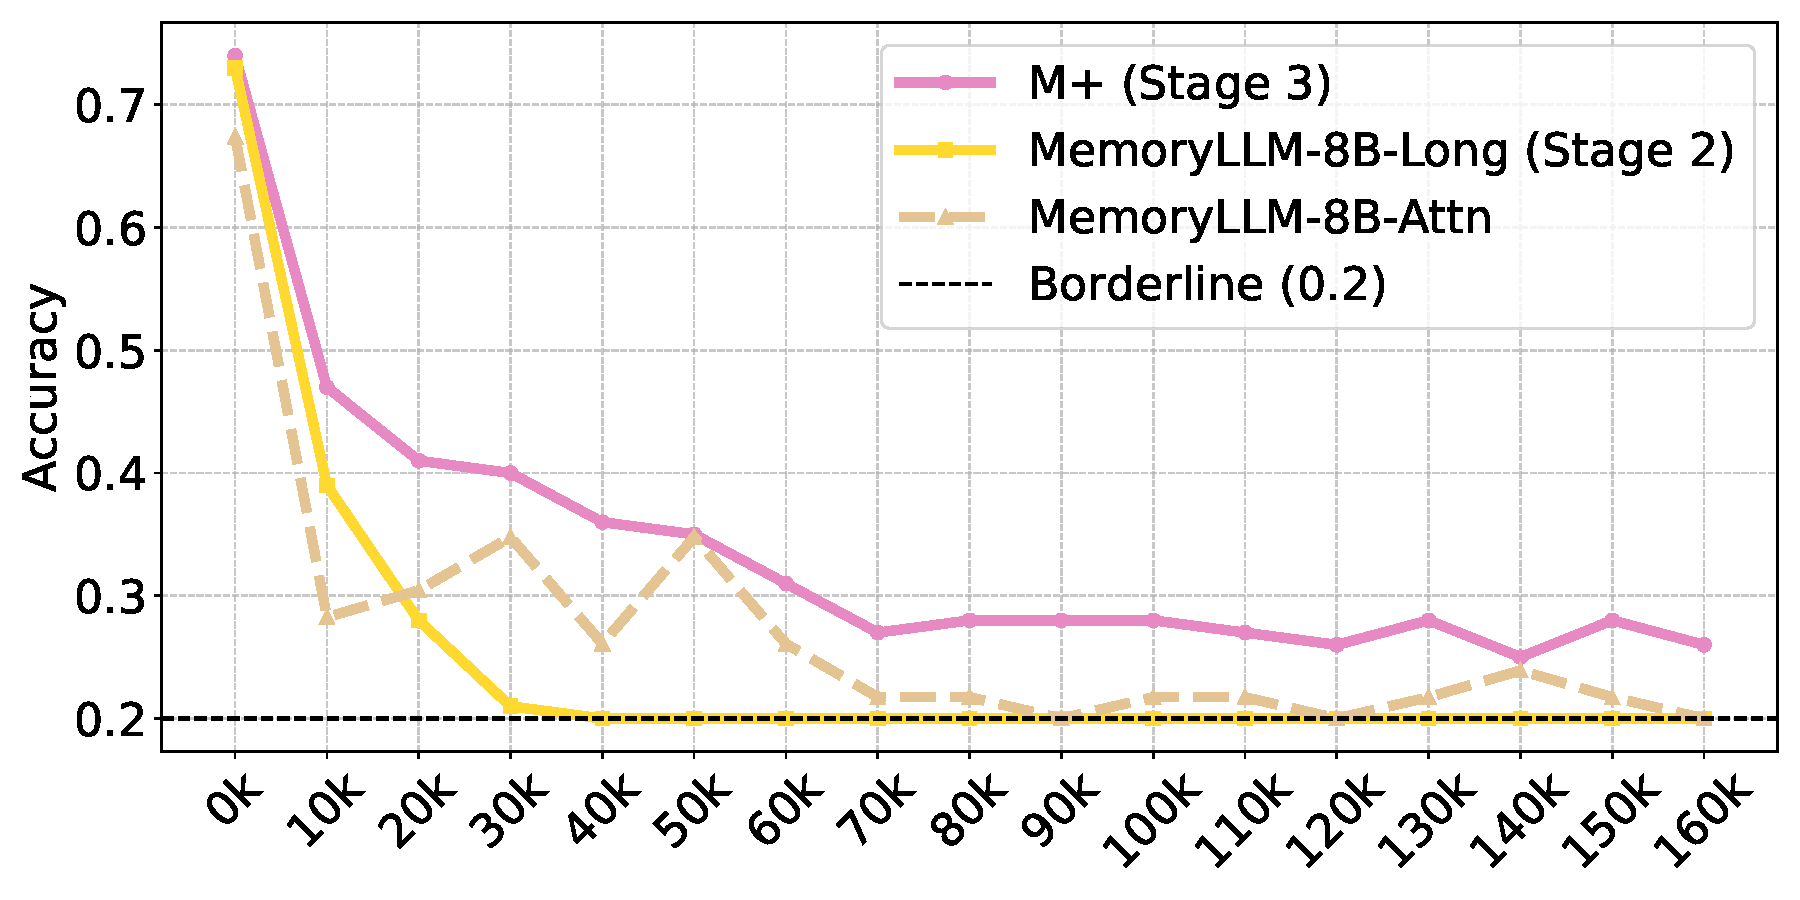
\includegraphics[width=0.6\linewidth]{figures/nqa_ablation.pdf}
    \caption{Ablation Study on NaturalQA dataset.}
    \label{fig:nqa_ablation}
\end{figure}

\section{Statistics of the Dataset of Long Documents}
\label{sec:statistics_of_long_documents}
We go through the whole dataset SlimPajama-627B and extract all dataset that have more than 4k tokens using the tokenizer of Llama-3.1-8B. The statistics are shown in Table \ref{tab:sequence-ranges}. We show six categories here (4k-8k, 8k-16k,16k-32k,32k-64k,64k-128k,128k+) but we only use the data within the first four categories (4k-8k, 8k-16k,16k-32k,32k-64k). This is because the examples longer than 64k are mainly from the category \textbf{Book} and lack diversity. 


\begin{table}[htbp]
\centering
\small
\resizebox{\textwidth}{!}{
\begin{tabular}{llrrrrrrr}
\toprule
\textbf{Range} & \textbf{Total} & \textbf{CommonCrawl} & \textbf{GitHub} & \textbf{ArXiv} & \textbf{C4} & \textbf{StackExch.} & \textbf{Wikipedia} & \textbf{Book} \\
\midrule
\textbf{4k--8k} & 11{,}189{,}999 
               & 7{,}759{,}741 (69.35\%) 
               & 692{,}224 (6.19\%) 
               & 286{,}537 (2.56\%) 
               & 1{,}825{,}018 (16.31\%) 
               & 142{,}457 (1.27\%) 
               & 481{,}854 (4.31\%) 
               & 2{,}168 (0.02\%) \\
\textbf{8k--16k} & 4{,}706{,}687 
                & 3{,}273{,}619 (69.55\%) 
                & 270{,}369 (5.74\%) 
                & 550{,}192 (11.69\%) 
                & 439{,}143 (9.33\%) 
                & 20{,}284 (0.43\%) 
                & 146{,}545 (3.11\%) 
                & 6{,}535 (0.14\%) \\
\textbf{16k--32k} & 1{,}607{,}064 
                 & 968{,}714 (60.28\%) 
                 & 95{,}445 (5.94\%) 
                 & 423{,}401 (26.35\%) 
                 & 70{,}223 (4.37\%) 
                 & 1{,}510 (0.09\%) 
                 & 34{,}323 (2.14\%) 
                 & 13{,}448 (0.84\%) \\
\textbf{32k--64k} & 443{,}438 
                 & 224{,}168 (50.55\%) 
                 & 32{,}653 (7.36\%) 
                 & 146{,}582 (33.06\%) 
                 & 3{,}413 (0.77\%) 
                 & 102 (0.02\%) 
                 & 5{,}940 (1.34\%) 
                 & 30{,}580 (6.90\%) \\
\textbf{64k--128k} & 192{,}515 
                  & 72{,}583 (37.70\%) 
                  & 11{,}753 (6.10\%) 
                  & 27{,}942 (14.51\%) 
                  & 38 (0.02\%) 
                  & 5 (0.00\%) 
                  & 507 (0.26\%) 
                  & 79{,}687 (41.39\%) \\
\textbf{128k+}    & 98{,}097 
                  & 23{,}721 (24.18\%) 
                  & 4{,}523 (4.61\%) 
                  & 5{,}167 (5.27\%) 
                  & 0 (0.00\%) 
                  & 2 (0.00\%) 
                  & 49 (0.05\%) 
                  & 64{,}635 (65.89\%) \\
\bottomrule
\end{tabular}}
\caption{Number of examples by sequence-length range and source (counts and percentages).}
\label{tab:sequence-ranges}
\end{table}


\section{Additional Training Details}
% \subsection{Details of Training Sub-Tasks}
\label{sub:details_of_training_sub_tasks}
In our training, we follow MemoryLLM~\citep{memoryllm} and design three sub-tasks:
\begin{itemize}
    \item \textbf{Two-Chunk Training}: Given a document split into two chunks $(x_1, x_2)$, we inject $x_1$ into the memory and update the transformer $\phi$ using the loss on $x_2$. Notably, we retain the gradients across both forward passes. 
    \item \textbf{Multi-Chunk Training}: For documents with multiple chunks $(x_1, \dots, x_n)$, we inject $x_1, \dots, x_{n-1}$ into the memory while detaching gradients, then update $\phi$ using the loss on $x_n$.
    \item  \textbf{Revisiting Cached Chunks}: Since the memory is continually updated during training, we cache the last chunk $x_n$ of earlier documents and revisit it periodically. When revisiting $x_n$, there are already many chunks injected between $x_1, \cdots, x_{n-1}$ and $x_n$. We denote the number of injected chunks between $x_{n-1}$ and $x_n$ as \emph{revisit distance}. We carefully tune the probability of deleting and updating the cache after each training step, and we manage to maintain the average revisit distance to be around 60 for Stage 1 \& Stage 2, and maintain the average distance to be around 200 for Stage 3. 
\end{itemize}


\section{Discussions}
\subsection{Similarities to Attention-Based Retrieval Methods}
\label{sub:attention_based_retrieval_methods}
In \ours, we use a co-trained retriever to retrieve the hidden states. In this process, we acknowledge that our method shares some similarities with prior approaches that use attention to retrieve keys and values. However, there are critical differences that make our approach unique and practically advantageous: 
\begin{itemize}
    \item  \textbf{Efficiency}: Methods such as SnapKV maintain and retrieve key-value pairs per head, which becomes extremely costly when scaled. In our setting—with 32 layers and 32 attention heads per layer—this requires 1024 retrievals per query, resulting in significant latency (as noted in line 59 of our paper). In contrast, M+ uses a co-trained retriever to retrieve memory tokens, which are compressed hidden states. This results in only 32 total retrievals—one per layer—dramatically reducing both computational cost and latency.
    \item \textbf{Performance}: In Figure 6, the curve labeled MemoryLLM-8B-Attn follows the SnapKV-style approach of retrieving key-value pairs using attention per head. As shown in the figure, it performs substantially worse than M+, highlighting that our co-trained retriever not only improves efficiency but also yields better results in practice compared with attention-based retrievals.
    \item \textbf{Design}: Note that our training setup includes both relevant and irrelevant documents (See details in Appendix \ref{sub:details_of_training_sub_tasks}), making it well-suited for contrastive learning. This allows us to effectively train the retriever, which integrates naturally into our overall training framework.
\end{itemize}

\subsection{The Form of Long-Term Memory (Hidden States vs. KV)}
\label{sub:form_of_long_term_memory}
In our work, we choose the use hidden states as the latent-space memory instead of key-value (KV) caches. This is based on the following two considerations: 
\begin{itemize}
    \item \textbf{Compression Efficiency}: As detailed in the paper, we compress each 512-token chunk into 256 memory vectors per layer in a lossless manner. In contrast, KV-based methods often require downsampling—e.g., dropping half the keys and values—to control memory size, resulting in unavoidable information loss. 
    \item \textbf{Retrieval Efficiency and Performance}: As described above, hidden states can be effectively retrieved using our co-trained retriever, requiring only 32 retrievals for each query. In contrast, a KV-cache approach would demand up to 1024 retrievals, significantly increasing computational cost. Furthermore, as shown in Figure 6, using hidden states yields better performance compared to using KV caches.
\end{itemize}



\subsection{Latency and Memory Consumption while Scaling}
\label{sec:latency_and_memory_consumption_while_scaling}
We aim to discuss the scalability of \ours by analysing the latency and memory consumption when scaling up. 
Theoretically, the end-to-end \emph{retrieval latency} scales linearly with three key variables:

\begin{enumerate}[label=(\arabic*)]
    \item Hidden size of the retriever, denoted by $d$.  
          In \textsc{M+}, we set $d = 256$, whereas the base model uses $d = 4096$.
    \item Size of long-term memory, denoted by $s$.  
          We cap this at 150k entries.
    \item Number of transformer layers, denoted by $L$.  
          For \textsc{LLaMA-3-8B}, $L = 32$.
\end{enumerate}

Hence,
\[
\text{latency} \;\propto\; d \, s \, L.
\]

Because we hold the long-term memory size $s$ fixed when scaling the model, $s$ is effectively a constant:

\[
\text{latency} \;\propto\; d \, L.
\]

Both $d$ and $L$ grow with the model size $M$, following
\[
M \;\propto\; d \, L,
\]
which implies a \textbf{linear relationship} between retrieval latency and model size:
\[
\text{latency} \;\propto\; M.
\]

\paragraph{Concrete Example} Scaling from \textsc{LLaMA-3-8B} ($d=4096$, $L=32$) to \textsc{LLaMA-3-70B} ($d=8192$, $L=80$) yields
\[
\frac{8192 \times 80}{4096 \times 32} \;=\; 5,
\]
i.e.\ a $\sim\!5\times$ increase in retrieval latency.  
For comparison, the parameter count rises by
\(
\frac{70\text{B}}{8\text{B}} \approx 8.75\times,
\)
showing that latency scales roughly linearly—rather than quadratically—with model size.

\paragraph{Memory Consumption} The extra \emph{memory overhead} from our method arises solely from the introduced memory tokens.  
This overhead also scales linearly with both $d$ and $L$; thus, the move from \textsc{LLaMA-3-8B} to \textsc{LLaMA-3-70B} incurs an analogous $\sim\!5\times$ increase in memory usage, mirroring the latency scaling.


\subsection{FLOPs Comparison}
\label{sub:flops_comparison}
We report the total FLOPs for generating one token after processing a sequence of varying lengths (from 2k to 128k), using a single H100 GPU. We employ the \texttt{torch.profiler} library to capture FLOPs during inference. The results are as follows:

\begin{center}
\begin{tabular}{c|cc}
\toprule
\textbf{Sequence Length} & \textbf{LLaMA-3.1-8B} & \textbf{M+} \\
\midrule
2048    & $5.68 \times 10^{13}$ & $6.92 \times 10^{13}$ \\
4096    & $1.13 \times 10^{14}$ & $1.32 \times 10^{14}$ \\
8192    & $2.26 \times 10^{14}$ & $2.55 \times 10^{14}$ \\
16384   & $4.48 \times 10^{14}$ & $5.01 \times 10^{14}$ \\
32768   & $8.88 \times 10^{14}$ & $9.86 \times 10^{14}$ \\
65536   & $1.75 \times 10^{15}$ & $1.94 \times 10^{15}$ \\
131072  & \texttt{OOM}          & $3.78 \times 10^{15}$ \\
\bottomrule
\end{tabular}
\end{center}

From the results, we observe that M+ and LLaMA-3.1-8B exhibit comparable FLOPs across all tested sequence lengths. Notably, while LLaMA-3.1-8B runs out of memory (\texttt{OOM}) at the 128k setting, M+ remains functional, highlighting its superior scalability for long-context inference.


\subsection{Interpretability of Memory Vectors}
\label{sub:interpretability_of_memory_vectors}
Our memory vectors can be viewed as hidden states within the transformer layers, with the key difference being that they may store more \textbf{compressed} information due to their persistent role across sequences. As such, the type of information they capture should be similar to the representations observed in the intermediate layers of a transformer when processing text.

Across layers, we hypothesize that the memory vectors follow a similar pattern to what has been reported in prior work on transformer interpretability~\cite{jawahar2019does, simoulin2021many}:
\begin{itemize}
    \item \textbf{Lower layers} tend to encode more \textbf{surface-level features},
    \item \textbf{Higher layers} tend to encode more \textbf{semantic or abstract information}.
\end{itemize}

Regarding long-term memory, it is constructed by \textbf{randomly dropping} vectors from the short-term memory and storing them for extended use. Importantly, long-term memory vectors are structurally \textbf{identical} to short-term ones. This means that, at any point, \textit{swapping a vector between long-term and short-term memory has no immediate effect} on model behavior.

In essence, the long-term memory acts as a \textbf{cache} that helps memory vectors \textbf{persist over time} rather than being overwritten too quickly.


